\section{Pruebas preliminares}

\begin{figure}
    \centering
    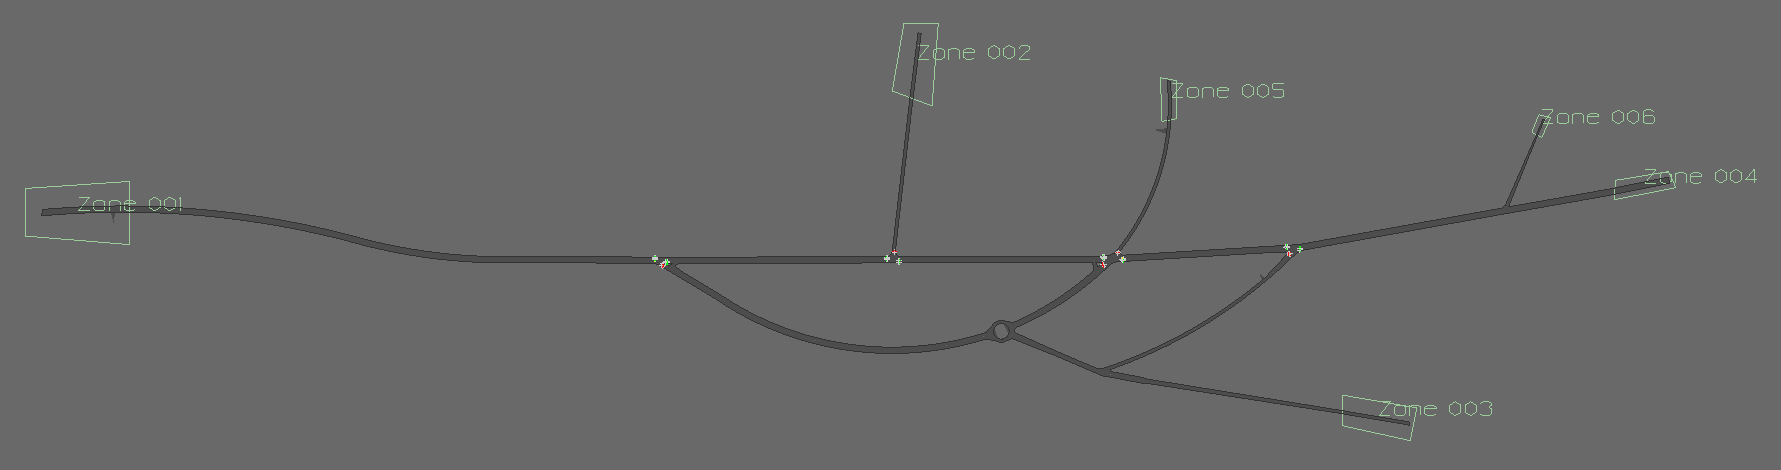
\includegraphics[width=\linewidth]{figuras/network8.png}
    \caption{Red de transporte utilizada para las pruebas preliminares.}
    \label{fig:network8}
\end{figure}

La validación preliminar del \emph{framework} se realizó utilizando la implementación de TraCI en Python incluída en la distribución de SUMO. Esta consiste en una librería para Python 2+ y 3+, la cual implementa un cliente TraCI en su totalidad (\autocite{pytraci, pytracisrc}), permitiendo así la validación del correcto funcionamiento de los comandos implementados en el \emph{framework} PVeins.

Por otro lado, la red de transporte utilizada para las pruebas corresponde a una red simple, incluida por defecto en la instalación de Paramics. Esta red consiste en un corredor central y conjunto de calles que lo intersectan (ver figura \ref{fig:network8}). El flujo de vehículos en la red es medio-bajo, manteniéndose bajo los 500 vehículos activos en cualquier momento dado.

A lo largo del desarrollo de este trabajo, se utilizó la librería anteriormente mencionada, junto con el entorno de \emph{debugging} de Visual Studio y la red de transporte, para probar la correcta implementación de cada funcionalidad que se le agregó al \emph{framework}. Se implementaron simples \emph{scripts} en Python para probar cada una de las funcionalidades desarrolladas; sólo se utilizará uno de éstos como ejemplo a continuación, ya que no es factible ni interesante exponer todas las pruebas realizadas en este documento, dada la gran cantidad de éstas que se efectuaron y alto grado de similitud que existe entre las mismas.

\subsection{Ejemplo de script de prueba: cambio de ruta}

El código \ref{code:py_routechange} expone el \emph{script} utilizado para una prueba de la funcionalidad del cambio de ruta en TraCI, funcionalidad que fue implementada en la última etapa de desarrollo del software, por lo que ya se contaba con una base con más funcionalidades sobre la cual construir (\emph{e.g.}, obtención de valores mediante suscripciones).

Este código expone de manera clara la estructura del \emph{loop} de simulación TraCI, estructura que se replica en VEINS (aunque de manera mucho más compleja); el cliente es quien controla la ejecución de los pasos de simulación, avanzando el escenario a medida que va realizando sus propios cálculos y análisis.

\lstinputlisting[style=MyPython, caption={Ejemplo de prueba, cambio de ruta.}, label={code:py_routechange}]{codigo/pytraci_routechange.py}